\section{Methods} \label{sec:methods}%
In this section, we describe the set of numerical experiments designed
to investigate the fundamental fluid dynamics associated with
acoustically-accelerated, perturbed liquid-gas interfaces.

\subsection{Problem set-up}
\label{subsec:setup}
\begin{figure}
  \centering
  \def\svgwidth{0.48\textwidth}
  \import{./figs/lung_figs/}{usbe_lung_schematic2.pdf_tex} \hfill%
  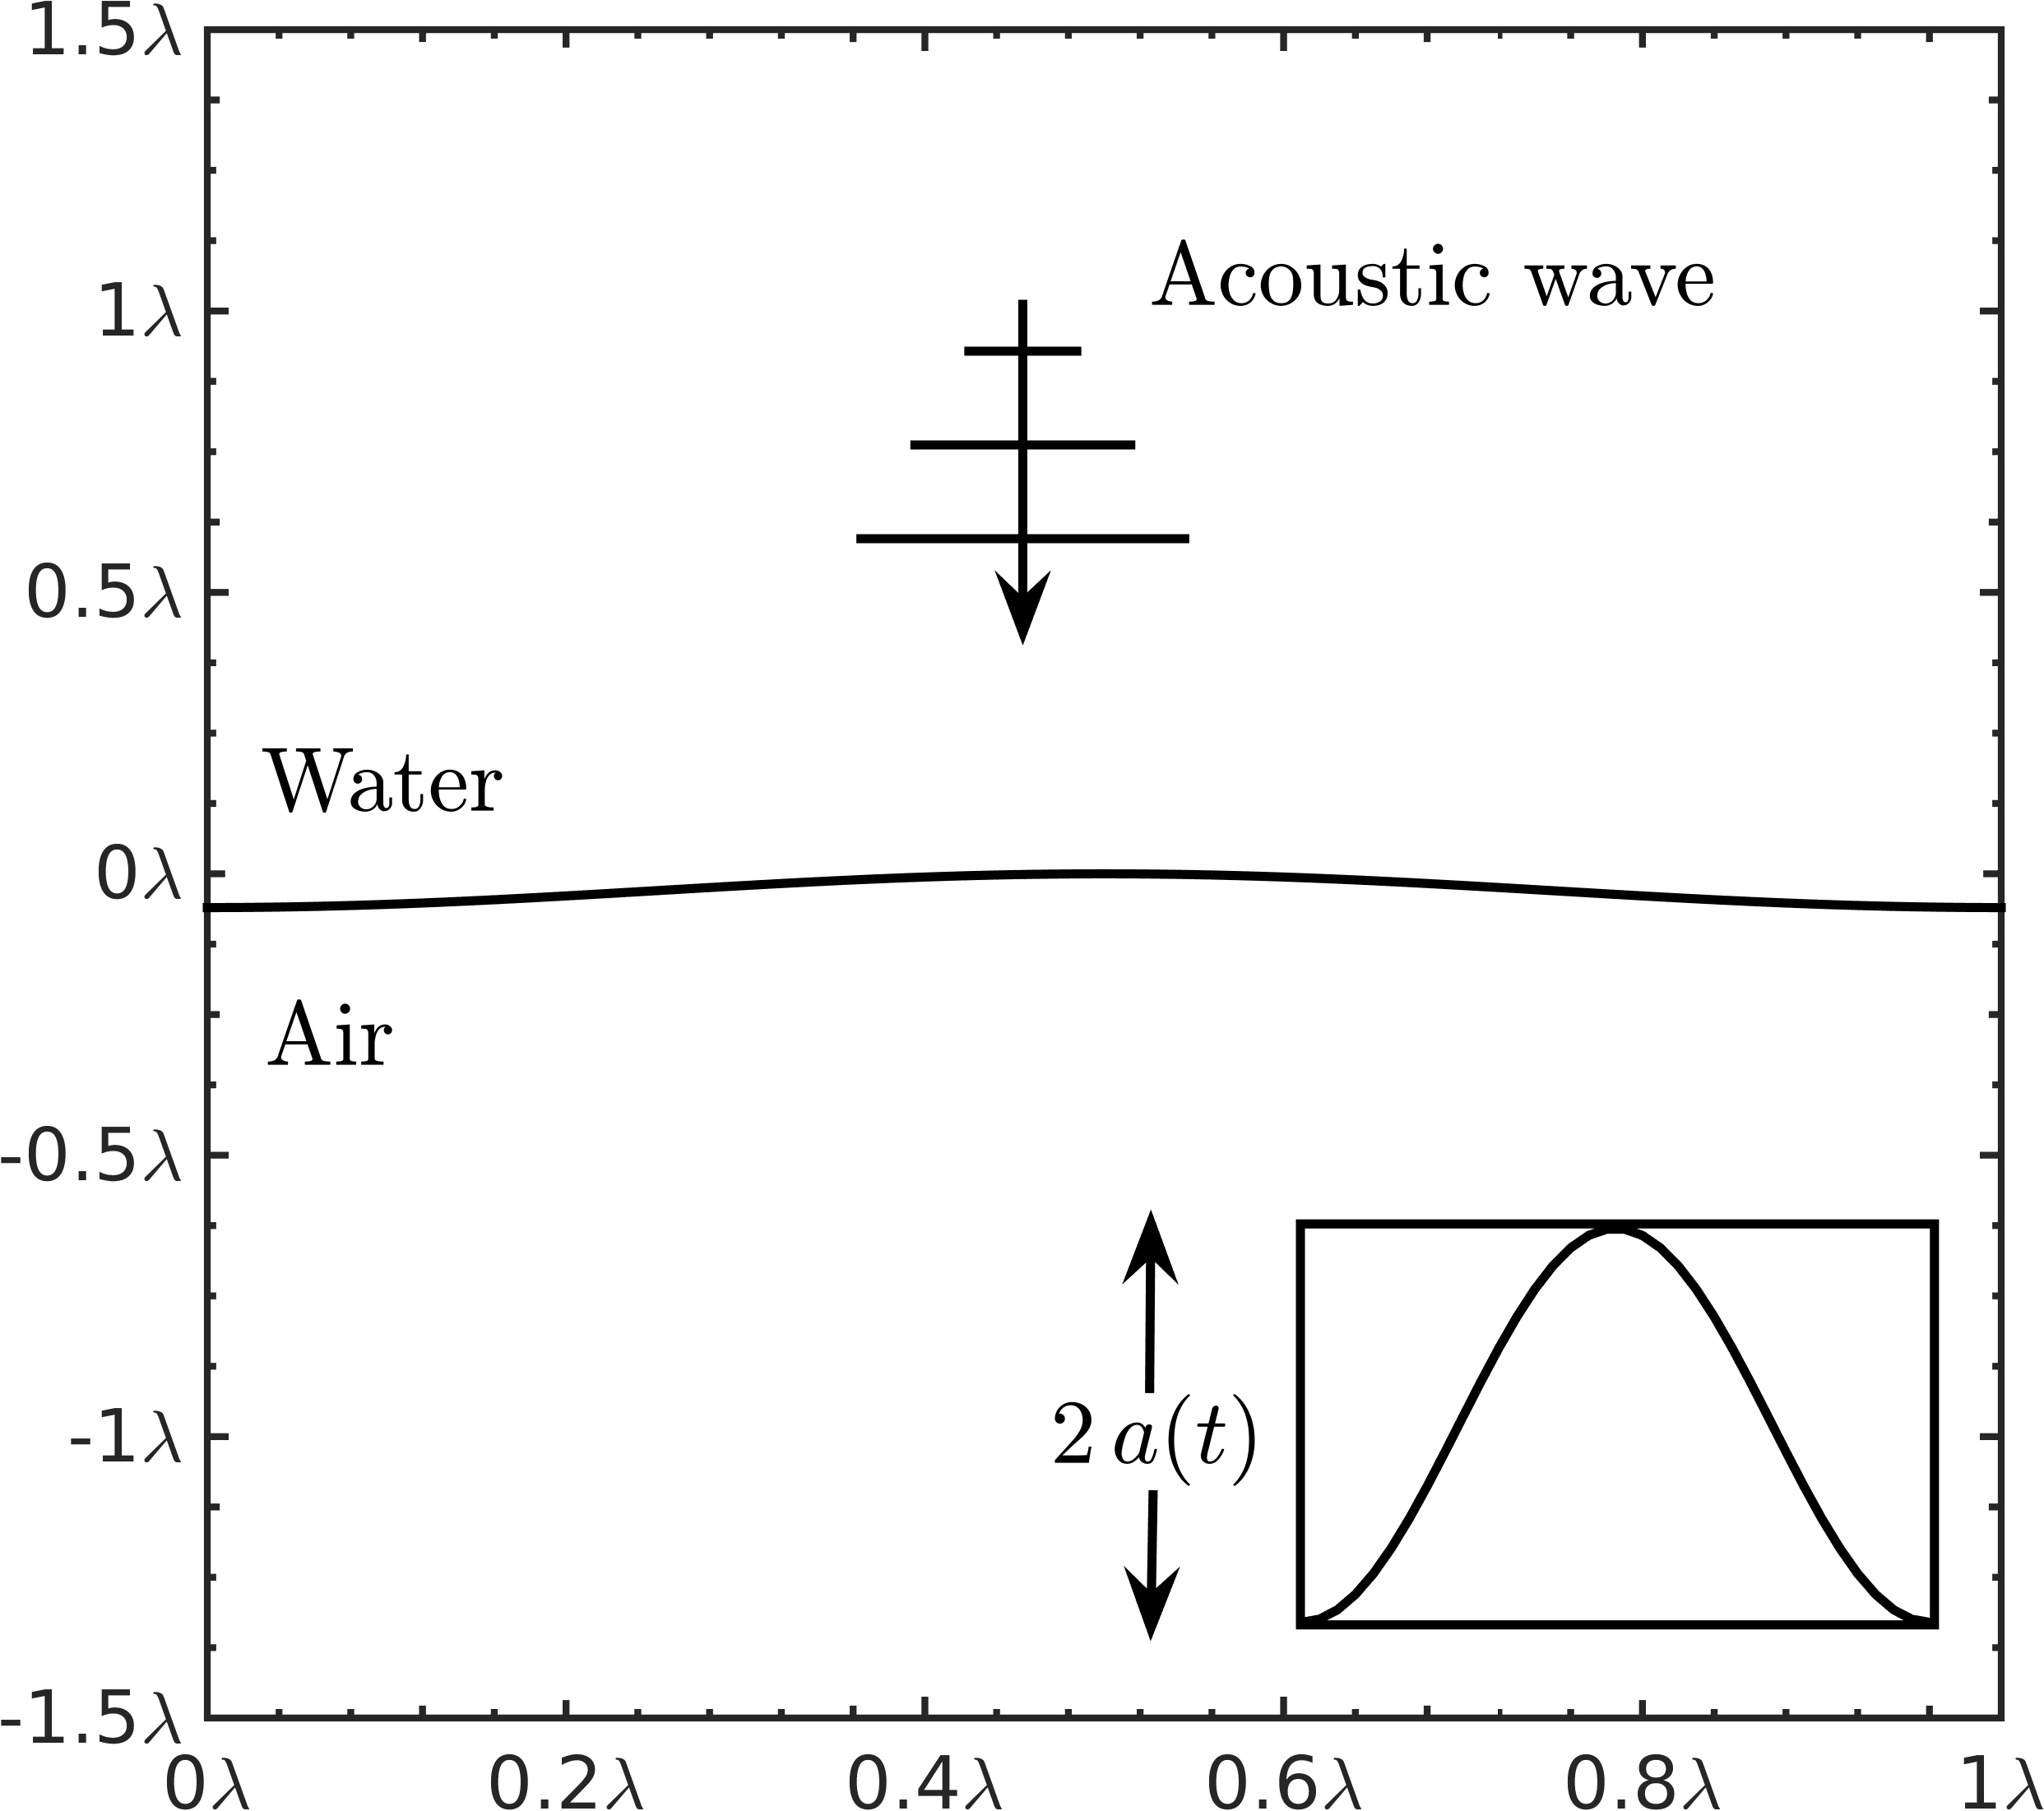
\includegraphics[width=0.48\textwidth]{./figs/lung_figs/usbe_model_schematic2} \hfill
  \caption[A schematic view of the model problem]{A schematic of an
    ultrasound wave impinging upon an alveolus (Left) is modeled as a sinusoidally perturbed water-air interface with an acoustic wave impinging from water onto the interface (Right).}
  \label{fig:problem_schematic}
\end{figure}
% 
We consider a 2D, compressible inviscid fluid system in the $xy$-plane
with an acoustic wave impinging from water (top) downward toward air
(bottom). The water-air interface is initially located at the origin
and has a sinusoidal shape with wavelength $\lambda$ and amplitude
$0.03\lambda$ as seen in Figure \ref{fig:problem_schematic}. The width
of the rectangular computational domain is $1\lambda$ such that it is
traversed by a single period of the interface. This interface geometry
is consistent previous studies of the \ac{RMI}
\citep{Brouillette2002}.

As the primary focus of this study is on the fundamental physics of
acoustically-accelerated perturbed liquid-gas interfaces a very simple
acoustic waveform that can be studied analytically is optimal for our
purposes. As such, we choose initially symmetric trapezoidal waveforms
for the numerical experiments as illustrated in Figure
\ref{fig:p0}. The wave is composed of three stages, described here in
the order that they encounter the interface. First, compression
occurs, the pressure increases linearly from atmospheric to a maximum
of $p_a=1, 5$, or $10$ MPa gauge pressure. Second, the elevated
pressure $p_a$ is held constant over a fixed period. Note
that the subscript $_a$ will be used from here on to denote properties
of the acoustic wave. Third, an expansion occurs and pressure
decreases linearly back to atmospheric pressure. The pressure rise and
fall initially occur over equal distances $5\lambda$, such that they
have constant, equal spatial slopes $\pm p_{a}/5\lambda$. Unless
otherwise stated, the period of constant pressure has length
$35\lambda$ and thus the total length $L$ of the incoming acoustic wave is
$45\lambda$.
% 
\begin{figure}% 
  \centering%
  \hfill
  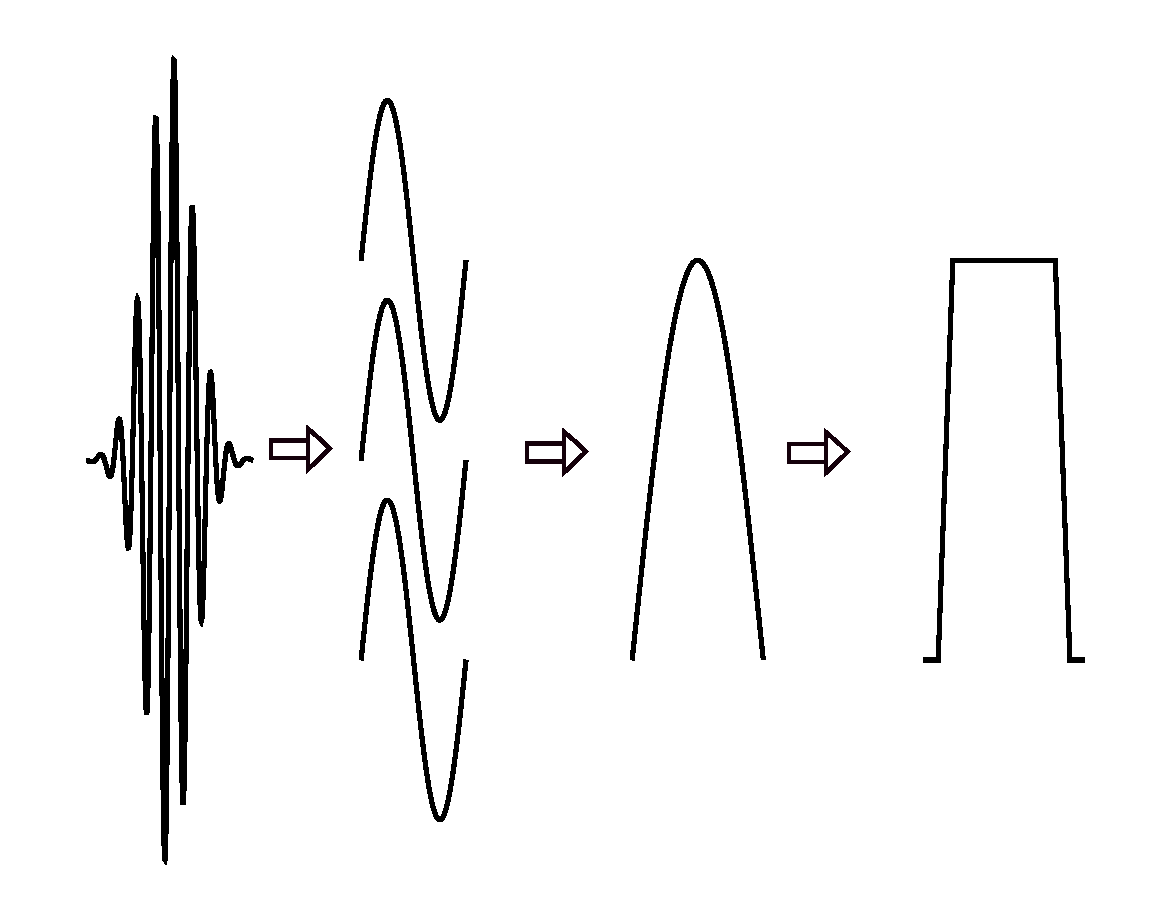
\includegraphics[width=0.3\textheight]{./figs/lung_figs/wave_logic_schematic}\hfill
  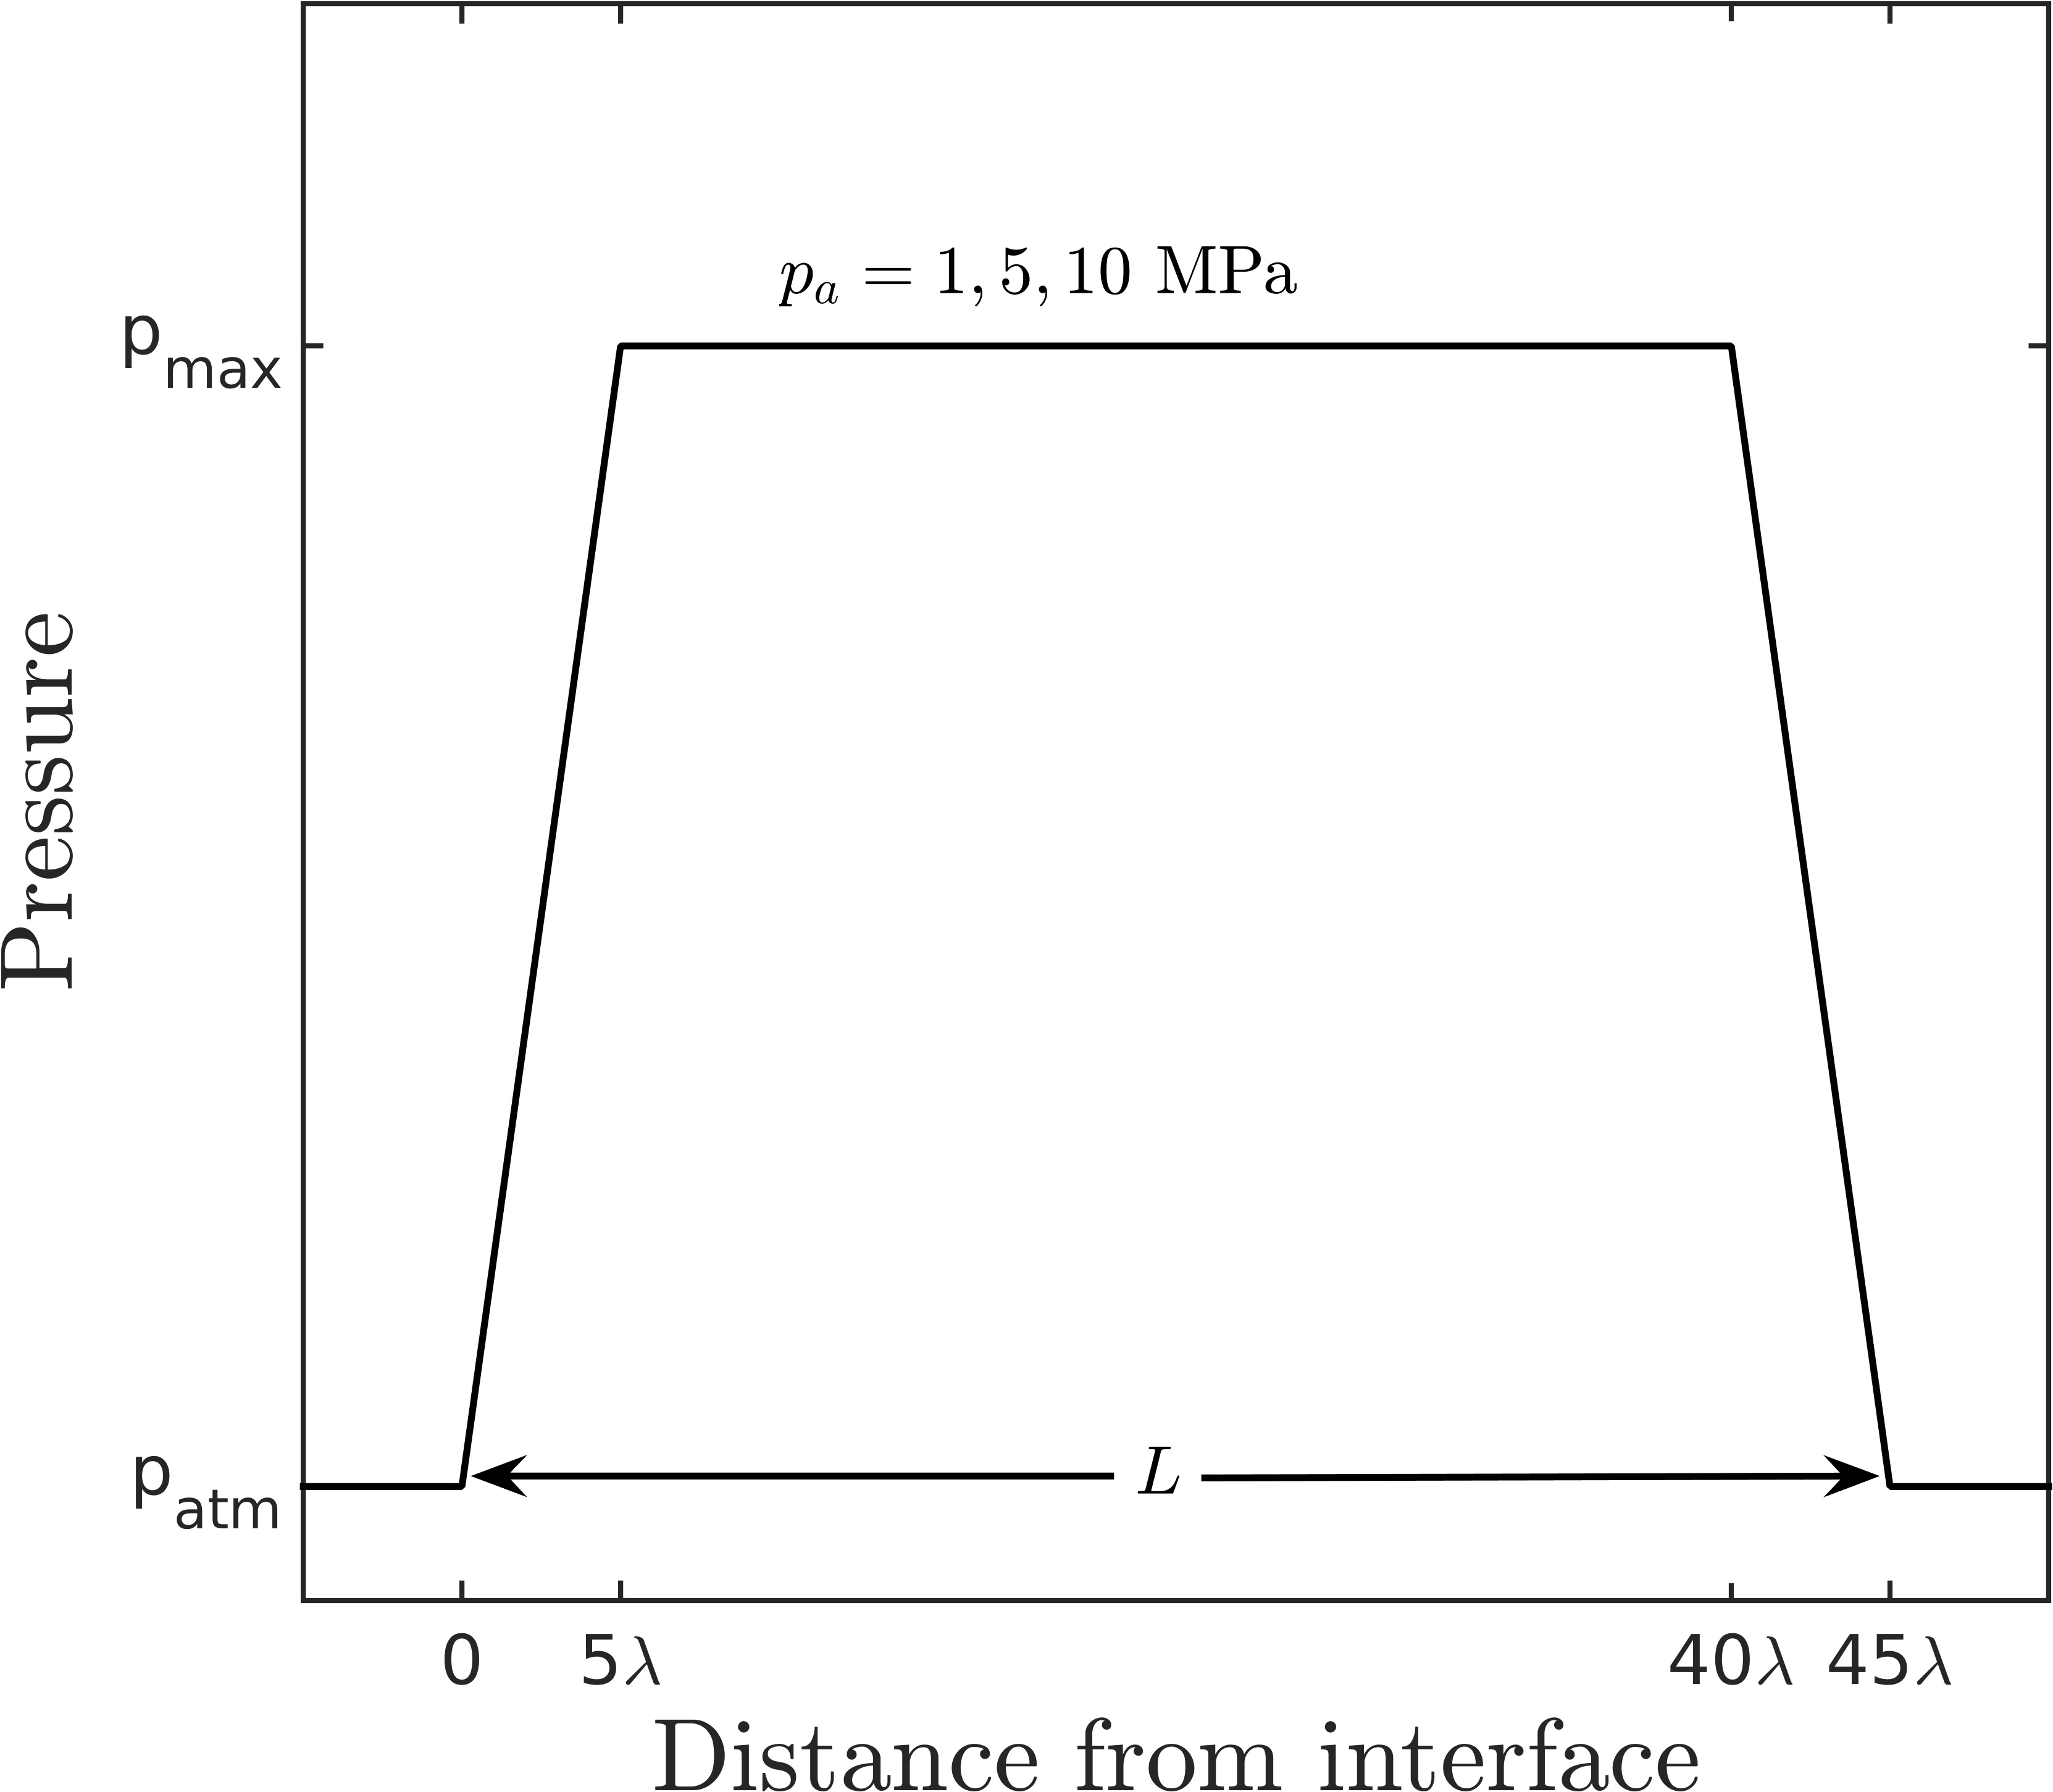
\includegraphics[width=0.3\textheight]{./figs/lung_figs/p0_vs_y_labeled}%
  \caption[Trapezoidal wave]{The ideological progression of how the
    trapezoidal wave was designed was is illustrated. The
    ultrasound pulse is thought of as a sum of sin waves, each of
    which is composed of half-sinusoids, which can be approximated as
    trapezoidal waves (Left). The specific trapezoidal pressure wave prescribed as an
    in initial condition is shown as a function of distance from the
    interface (Right).}%
  \label{fig:p0}
\end{figure}
% 
\subsection{Governing equations}
The governing equations describing the motivating problem of \ac{DUS}
of the lung are conservation of mass, momentum, and energy for a
compressible, viscoelastic material. The present work aims to
study the fundamental fluid physics of acoustically-accelerated,
perturbed liquid-gas interfaces, so we neglect elastic and viscous
effects. Hence We arrive at the Euler equations which we present here
for the case of fluid motion in two dimensions ($x,y$):
% 
\begin{subequations} \label{eq:euler}%
  \begin{align}% 
    \frac{\partial \rho}{\partial t} + \frac{\partial \left(\rho u\right)}{\partial x} + \frac{\partial \left(\rho v\right)}{\partial y} = 0,\\
    \frac{\partial \rho u}{\partial t} + \frac{\partial}{\partial x}\left( \rho u^2+p\right)  + \frac{\partial}{\partial y}\left( \rho uv\right) = 0,\\
    \frac{\partial \rho v}{\partial t} + \frac{\partial}{\partial x}\left( \rho uv\right)  + \frac{\partial}{\partial y}\left( \rho v^2+p\right) = 0,\\
    \frac{\partial E}{\partial t} + \frac{\partial}{\partial x}\left[u\left(E+p\right)\right] + \frac{\partial}{\partial y}\left[v\left(E+p\right)\right] = 0,
  \end{align}%
\end{subequations}%
% 
where $t$ is time, $\rho$ is density, $p$ is the pressure, $u$ and $v$
are the velocity components in the $x$ and $y$ directions
respectively, and $E$ is the total energy. We use the density and
sound speed of air at 300 K to nondimensionalize the system. It is
worth noting that the Euler equations are length scale invariant, and
thus no inherent physical length scale exists in the equations that we
solve. Hence all length scales hereafter will be considered relative
to an interface perturbation wavelength $\lambda$.

To close the system, we solve a stiffened equation of state which
relate the total energy to the pressure and velocity in the flow, such
that,
% 
\begin{align} \label{eq:stiffened_eos}%
  E=\frac{\rho\left(u^2+v^2\right)}{2} + \frac{p+\gamma B}{\gamma-1}.
\end{align}
% 
Here $B$ is a measure of liquid stiffness. For perfect gases, such as
is our treatment of air, $\gamma$ is the specific heats ratio and
$B=0$. The sound speed in our simulations is calculated based on the
following relationship, derived from the stiffened equation of state.
% 
\begin{align}
  c = \sqrt{\frac{\gamma\left(p+B\right)}{\rho}}.
\end{align}
% 
While physical diffusion is not considered in this setup, numerical
diffusion does occur at the water-air interface, creating a mixed
region between the two fluids. The numerical treatment of the
diffusion layer at the interface for the initial condition is such
that the density has an exponential profile \citep{Latini2007}, which
is used to get the mass fraction and molecular weight fields in the
mixed region. Which then used to determine the other material
parameters in the mixed region in a thermodynamically consistent
fashion.

To solve for
the material parameters in the mixed region and prevent spurious
pressure oscillations at the interface, two additional advection
equations are solved for $\gamma$ and $B$.
\begin{subequations} \label{usbe_lung_eosvar_advection}%
  \begin{align}% 
    \frac{\partial}{\partial t}\left(\frac{\gamma B}{\gamma-1}\right)+\vec{u}\frac{\partial}{\partial x}\left(\frac{\gamma B}{\gamma-1}\right) = 0,\\
    \frac{\partial}{\partial t}\left(\frac{1}{\gamma-1}\right)+\vec{u}\frac{\partial}{\partial x}\left(\frac{1}{\gamma-1}\right) = 0. 
  \end{align}%
\end{subequations}%
This implementation is consistent with the works of \cite{Abgrall1996,
  Shyue2001, Beig2015}. Details of the full numerical implementation
are explained by \cite{HenrydeFrahan2015}.
%
The dimensional and dimensionless values of each fluid property can be
found in tables \ref{tab:usbe_lung_dimensional_parameters} and
\ref{tab:usbe_lung_dimensionless_parameters} respectively.
% 
\begin{table}[bp]%
  \begin{center}
    \caption{Dimensional properties of air and water used in simulations.}
    \label{tab:usbe_lung_dimensional_parameters}%
    \begin{tabularx}{0.75\textwidth}{| X | X | X | X | X |}
      \hline
      & Density, $\rho^*$ (kg/m$^3$) & $\gamma$ & $B^*$ (Pa)  & $c^*$ (m/s) ($p$=$1$ atm) \\ \hline
      Air   & 1.18                        & 1.4      & 0         & 347.2     \\ \hline
      Water & 996                           & 5.5      & 492115000 & 1648.7     \\ \hline
      \multicolumn{5}{l}{\small $^*$ indicates dimensional parameter}
    \end{tabularx}
  \end{center}
\end{table}%
\begin{table}[bp]%
  \begin{center}
    \caption{Dimensionless properties of air and water used in simulations.}
    \label{tab:usbe_lung_dimensionless_parameters}%
    \begin{tabularx}{0.75\textwidth}{| X | X | X | X | X |}
      \hline
      & Density, $\rho$ & $\gamma$ & $B$ & $c$ \\ \hline
      Air   & 1                          & 1.4      & 0         & 1          \\ \hline
      Water & 846.6                      & 5.5      & 3469.1    & 4.75       \\ \hline
      \multicolumn{5}{l}{\small Parameters are nondimensionalized by the density and sound speed of air. }
    \end{tabularx}
  \end{center}
\end{table}
% 
\subsection{Numerical methods}%
\label{subsec:numerical_methods}%
To solve the governing equations, we implement a third-order accurate
\ac{DG} scheme in space and a fourth-order accurate, adaptive
Runge-Kutta method to march forward in time
\citep{HenrydeFrahan2015}. Roe solver is used to calculate flux in an
out of each cell in a way that handles discontinuities and keeps the
interface sharp. As previously stated, the computational domain width
($x$-direction) is $\lambda$. The domain length ($y$-direction) is
80$\lambda$. The grid resolution is 100 points per $\lambda$ unless
otherwise stated. To minimize artificial reflections, we use inflow
and outflow boundary conditions at the top and bottom of the domain,
and implement geometric grid stretching in the vertical direction for
the top and bottom-most 10$\lambda$ segments of the grid. Periodic
boundary conditions are used at the left and right edges of the
domain.

%%% Local Variables:
%%% mode: latex
%%% TeX-master: "../main"
%%% End:
